\chapter{Wikipedia}
\label{chp:wikipedia}
In this chapter, we provide an overview of the inner workings and decision making processes of Wikipedia. Firstly, in Section~\ref{sec:principles-wikipedia} we state the fundamental principles of Wikipedia and how it guides editors on the website. Next, we describe the roles and responsibilities of the  different categories of Wikipedia users in Section~\ref{sec:formal-org-wikipedia}. Lastly, we explain the election process for administrators and discuss the voting behaviour in terms of existing research. 

\section{Principles of Wikipedia}
\label{sec:principles-wikipedia}
Wikipedia is the largest online encyclopedia with over six million pages of content in the English version. It is maintained by an open collaborative effort of multiple editors from all across the world. All the knowledge and content is free and is supported by the non-profit Wikimedia Foundation. The size and popularity of Wikipedia is attributed to the ability for anyone to edit any content. All editors on Wikipedia follow five fundamental principles called the "Five Pillars" shown in Figure~\ref{fig:5-pillars}. 
These five pillars provide a foundational framework for collaboration amongst users and contribution towards the betterment of the Wikipedia project.  
\begin{figure}[!ht]
    \centering
    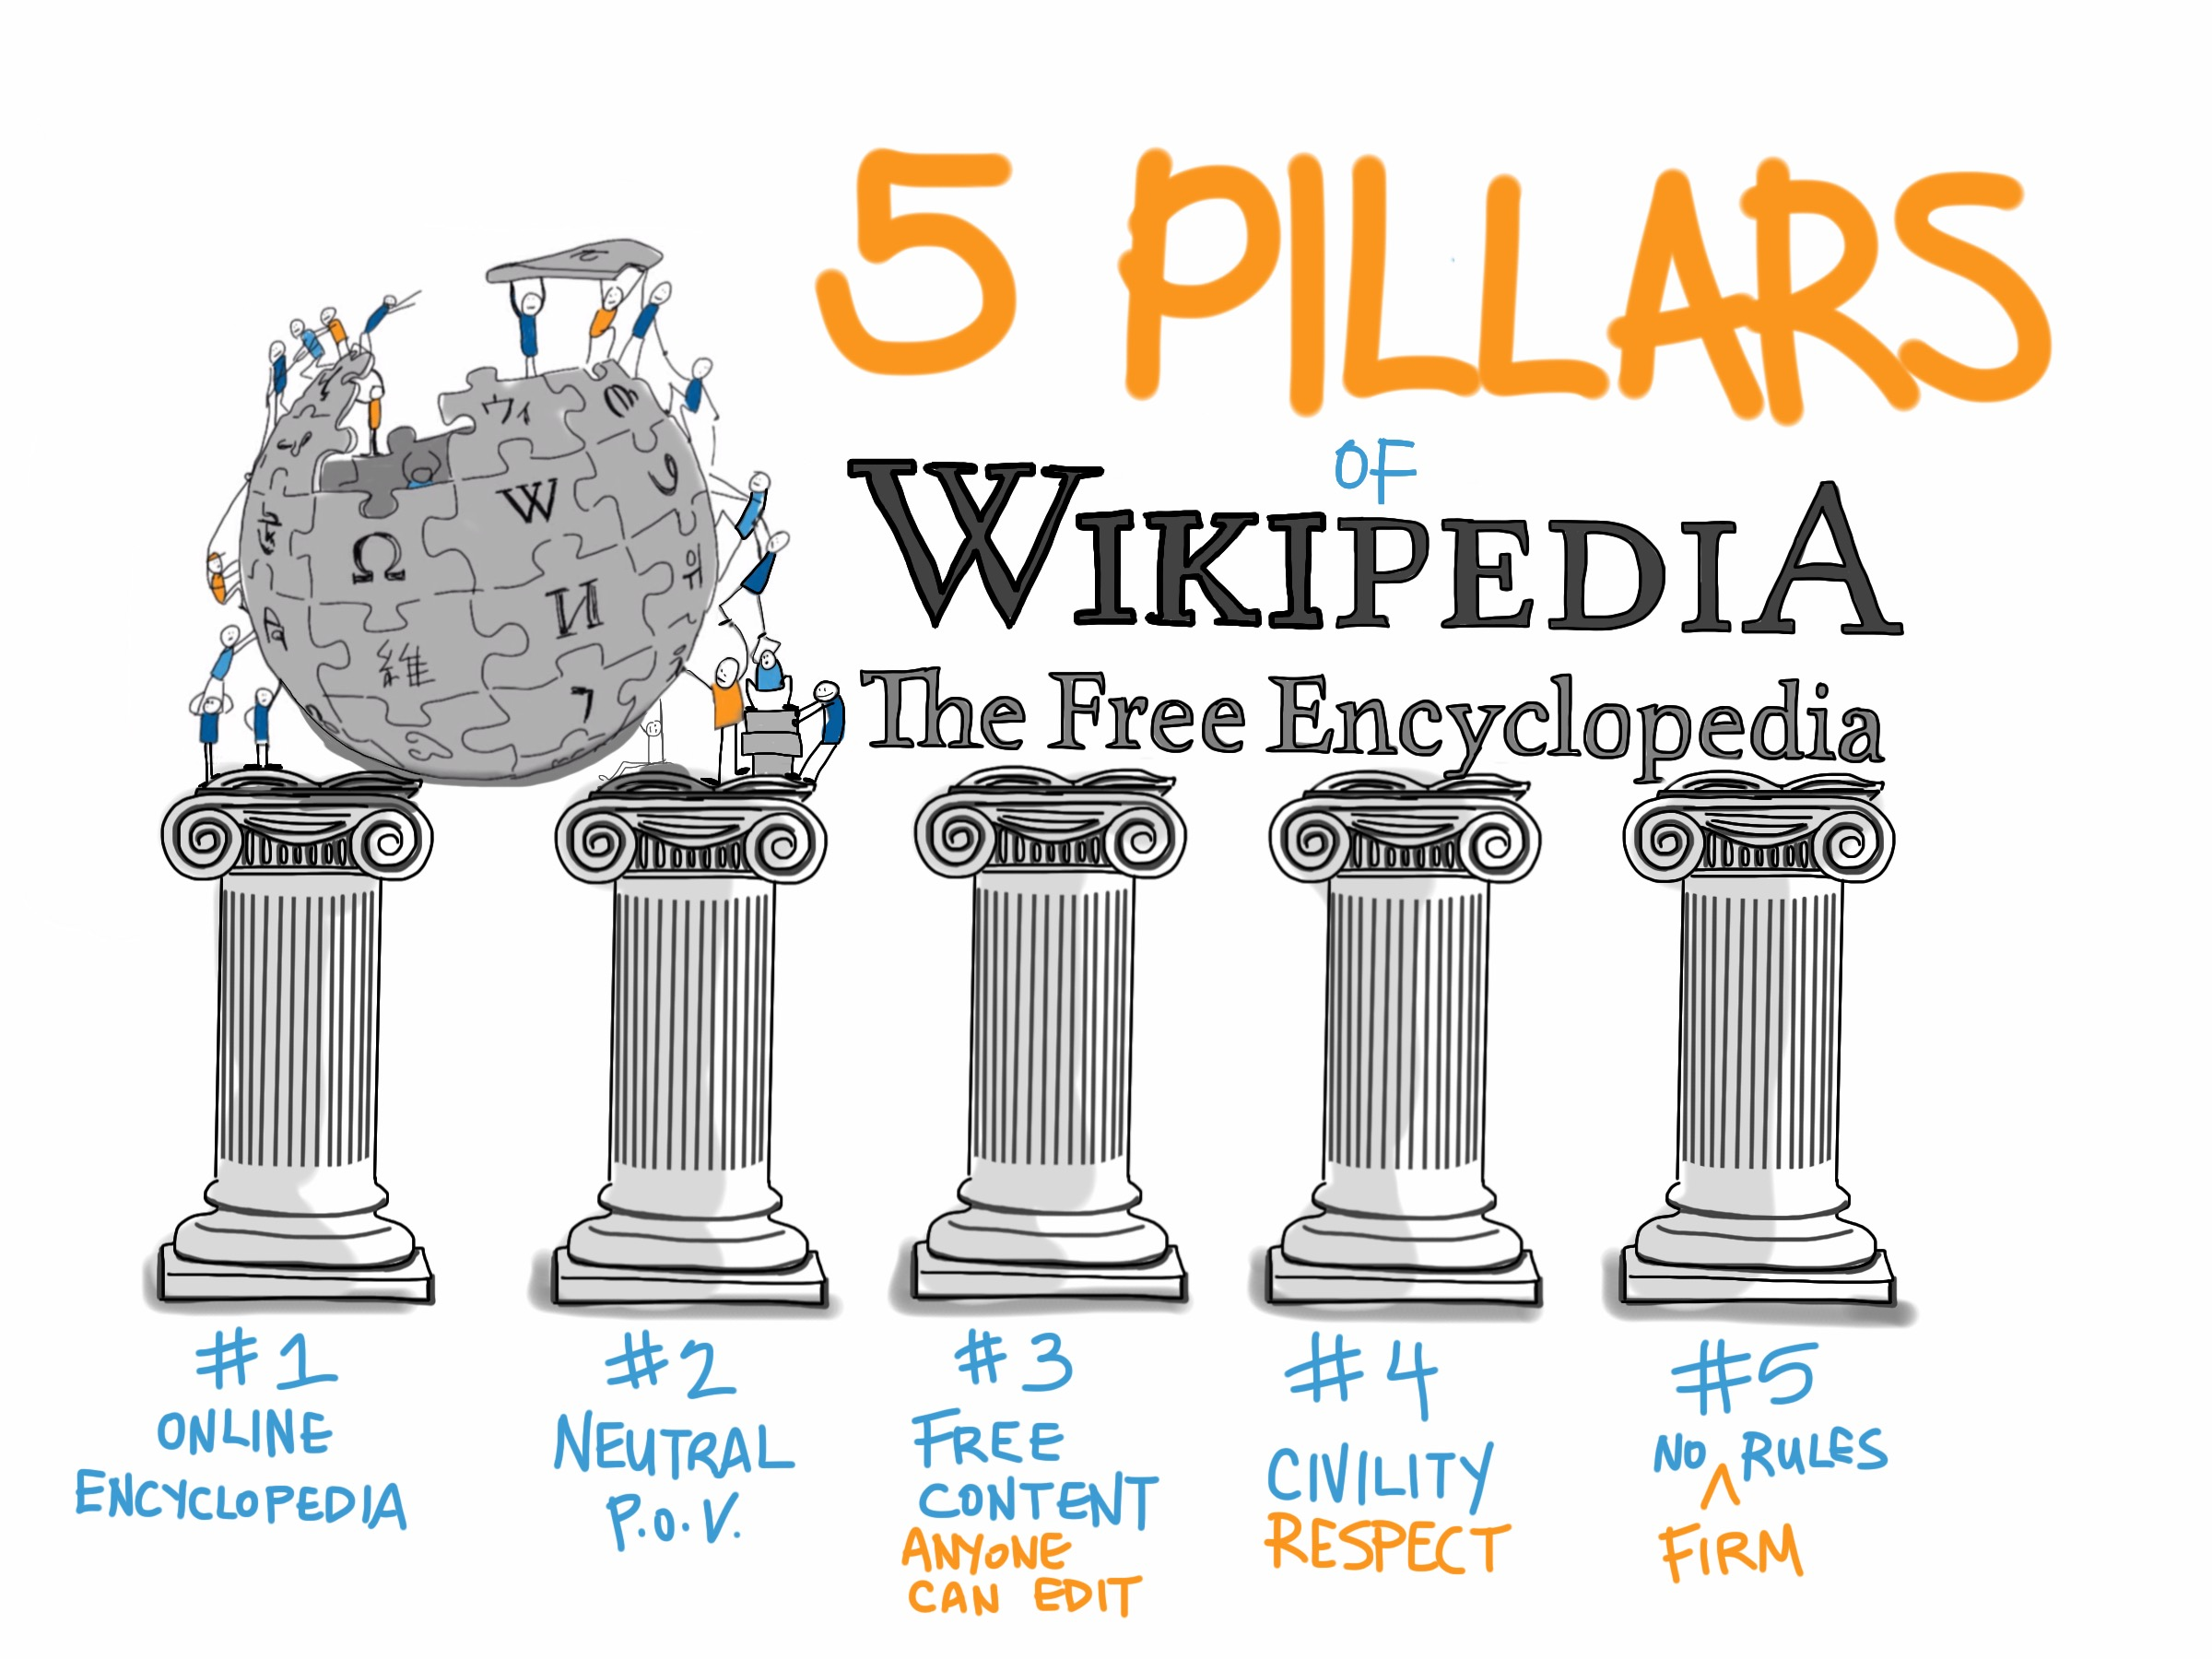
\includegraphics[width=0.75\textwidth]{images/Pillars.jpg}
    \caption{Five Pillars of Wikipedia. Image downloaded from \url{https://www.flickr.com/photos/gforsythe/21684596874}}
    \label{fig:5-pillars}   
\end{figure}

The first pillar states that Wikipedia is first and foremost an encyclopedia \cite{wiki:wiki-is-not}. Therefore, it must strictly not contain any original research, propaganda or advertisements \cite{wiki:wiki-NOR}. Materials that do not have reliable references will be removed by other edits.

The second pillar describes that articles on Wikipedia should strive to have a neutral point of view. This might include presenting multiple perspectives on the same subject accurately and not championing any one viewpoint as "correct" or "the truth". If disagreements are present then discussions must take place for building consensus.

The third principle enshrines the ideal that all content available on Wikipedia is free to edit and share. However, this does not mean copyrights and plagiarism is tolerated by the community. There is no ownership of an article by an editor; anyone may freely modify any content.

The fourth pillar describes Wikipedia's code of conduct. It asks users to act in good faith and assume good faith on the part of other editors. Wikipedia etiquette urges disputes and disagreements such as edit wars \cite{wiki:edit-wars}, to be resolved with civility while respecting other editors.

The fifth and last pillar reminds users that all rules in Wikipedia are essentially just policies and guidelines meant to help with collaboration. They can evolve and change to reflect the requirement of the community. It assuages the fear of making mistakes and encourages editors to be bold though not reckless. 

\section{Formal Organization of Wikipedia}
\label{sec:formal-org-wikipedia}
In this section, we describe the various categories of users and explain their roles and responsibilities. All the facts and figures we provide in this thesis are from the English version of Wikipedia. We define a "user" of Wikipedia as a person who contributes to the encyclopedia and a "reader" as someone who simply accesses the content.

Wikipedia started out as completely open with no restrictions on who can edit a page or create a new article. Changes and edits that were made to a page would be published immediately. This lead to many pages that contained erroneous text, biased content and gibberish. Therefore, this led to the English version of Wikipedia introducing restrictions and tools to protect the more controversial pages. They also introduced categories of users to help protect and maintain the quality of the content available on Wikipedia. We proceed to explain the four main user types as seen in Figure~\ref{fig:logos}. 
\begin{figure}[h!]
    \centering
    \begin{subfigure}[b]{0.49\textwidth}
        \centering
        
\includegraphics[width=0.5\textwidth]{images/wikipedians.jpg}
        \caption{Editors}
        \label{fig:editors}
    \end{subfigure}
    \begin{subfigure}[b]{0.49\textwidth}
        \centering
        
\includegraphics[width=0.5\textwidth]{images/admins.png}
        \caption{Administrators}
        \label{fig:admins}
    \end{subfigure}

    \begin{subfigure}[b]{0.49\textwidth}
        \centering
        
\includegraphics[width=0.5\textwidth]{images/bureaucrat.png}
        \caption{Bureaucrats}
        \label{fig:crats}
    \end{subfigure}
    \begin{subfigure}[b]{0.49\textwidth}
        \centering
        
\includegraphics[width=0.5\textwidth]{images/arbs.png}
        \caption{Arbitration Committee}
        \label{fig:arbs}
    \end{subfigure}
    \caption{Logos for each category of user that signifies the role that they play in the Wikipedia community.}
    \label{fig:logos}
\end{figure}

\subsection{Editors}
Editors (or Wikipedians) are the primary users who edit and create all the content on Wikipedia \cite{wiki:editors}. Figuratively, they hold Wikipedia in the palm of their hands as seen by the logo in Figure~\ref{fig:editors}. There are two main types of editors on Wikipedia namely, \textit{registered} and \textit{unregistered}. A registered user is one who has a unique username and a permanent \textit{talk page} where other can communicate with other users. An unregistered user is one who contributes without a registered username and are usually referred to as \textit{IPs} as they are only identified by their IP addresses. Unregistered users usually have similar rights as those of regular users to edit, discuss and contribute with certain exceptions 
\cite{wiki:unregistered-users}. Unregistered cannot create a new article, edit a protected page, become administrators or vote in elections to promote users within Wikipedia. As the focus of the thesis will be on the elections within Wikipedia, when we refer to editors in the coming chapters and sections we refer to the registered users.

There are over 38 million registered users and this number is constantly rising. However, only roughly $0.37\%$ ($\approx 144\,000$) of the total registered users are active, i.e., have performed some action in the past 30 days. An even smaller percentage of those active users participate in the community discussion forums on Wikipedia. Now, we will explain what tasks editors perform and how contribution is recorded in Wikipedia.

Each page in Wikimedia is classified into a \textit{namespace} based on the type of information that page contains \cite{wiki:namespace}. Namespaces separate pages into sets to distinguish content pages from administrative or editor related pages. For e.g, the \mainNS (or \articleNS) namespace contains all the encyclopedic content and the \userNS namespace contains the user pages and information related to their user accounts. Each page in Wikipedia also has a corresponding \textit{talk page}, which are used by editors to discuss changes to the page in question. For e.g., the \usertalkNS namespace has talk pages corresponding to each user page and acts as a system to message particular users. Figure~\ref{fig:namespace} shows a list of the subject namespaces and their corresponding talk namespaces. Now, we define a \textit{user contribution} as any addition, deletion or modification of a page under any namespace in Wikipedia \cite{wiki:user-contribs}. Wikipedia collects and stores every user contribution so that it can track cases of vandalism and copyright infringement. 

\begin{figure}[htp]
    \centering
    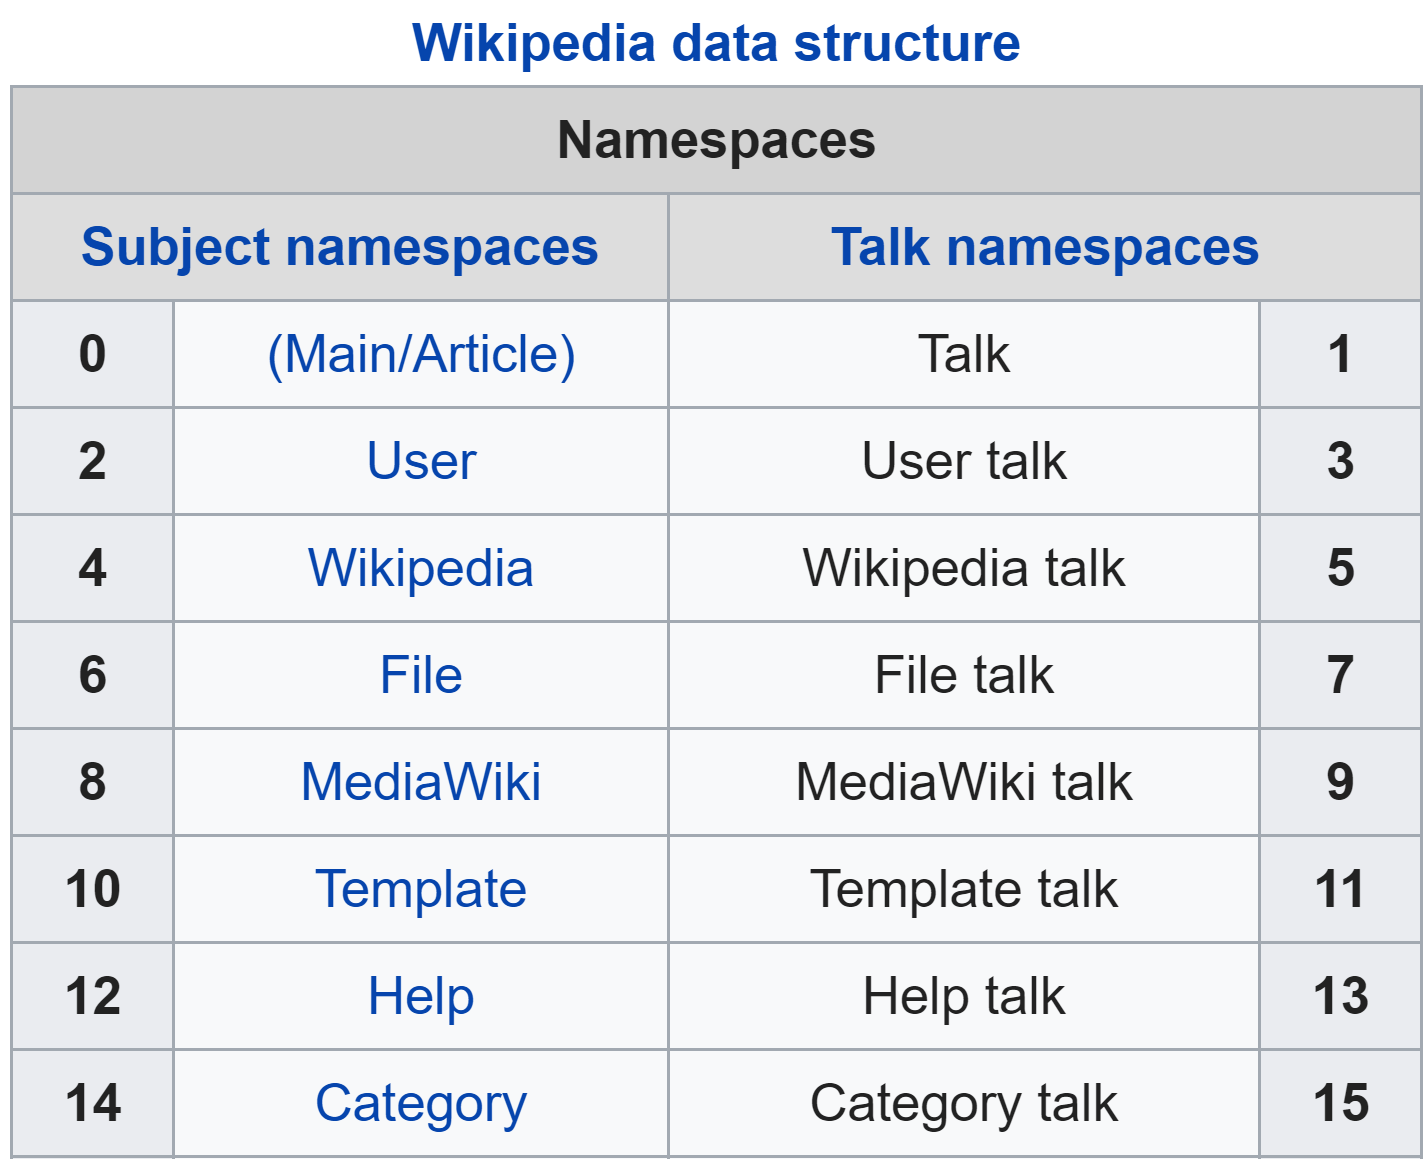
\includegraphics[width=0.75\textwidth]{images/namespaces.PNG}
    \caption{A list of the namespaces in Wikipedia \cite{wiki:namespace}.}
    \label{fig:namespace}
\end{figure}

The quality and quantity of the contribution of each editor varies significantly. There are many occasional users that just fix minor spelling and grammar errors in articles. At the same time, there are dedicated editors that constantly create new articles, update large portions of text, and include new references and images.   

\subsection{Administrators}
\textit{Administrators} (or \textit{admins}) are editors who are given access to certain tools and powers to maintain content on Wikipedia. Administrators can delete and restore deleted pages, block and unblock users and IP addresses from editing, protect and remove protection from sensitive pages \cite{wiki:admins}. These tools are associated with a mop that is used to clean up Wikipedia and is represented by their logo seen in Figure~\ref{fig:admins}. 
There are currently 1\,141 administrators of whom 500 are active. Although admins have access to these tools, they are considered to be no more important than regular editors. Administrators are elected through a week long process called \textit{Request for Adminship} (RfA) at the end of which successful candidates are instated by a Bureaucrat. We will cover RfA process in detail in the coming sections. 

Along with the tools and power, administrators also have certain responsibilities. They are not to misuse the tools at their disposal in conflicts or interest or disrupt Wikipedia by acting in bad faith. Administrators serve indefinitely, but can be removed  by Bureaucrats on the decision of the Arbitration Committee on the basis of abuse of powers or inactivity. Admins help with various areas of Wikipedia such as processing administrative backlogs, helping with ant-vandalism efforts, managing copyright issues, etc. 

\subsection{Bureaucrats}
\textit{Bureaucrats} (or \textit{Crats}) are users who perform certain actions \cite{wiki:bureaucrats}. They are usually administrators and oversee procedural rules and enforce decisions. There are a total of 19 bureaucrats currently in the English Wikipedia. Bureaucrats are involved in the granting or revoking of administrator status to users and adding and removing bots (software robots that carry out repetitive tasks on Wikipedia). Bureaucrats are bound by the policy and the consensus of the community in granting these roles or permissions and are, therefore, expected to be good arbiters of consensus. They are expected to be able to identify criteria for a "consensus" and also explain the reasons behind their actions when requested. 

Bureaucrats are also elected through a process similar to RfA called \textit{Request for Bureaucratship} (RfB), but usually demand higher thresholds of acceptance to be considered successful. Interestingly, Bureaucrats are also appointed following the final decision of another Bureaucrat, therefore, they have complete control over the whole process. However, a Bureaucrat cannot revoke the bureaucratic position of others. They also carry out the requests from the Arbitration Committee to remove permissions and privileges of admins or bots. As their name suggests Crats perform only bureaucratic duties and are therefore represented by the logo seen in Figure~\ref{fig:crats}.
\subsection{Arbitration Committee}



\section{Request for Adminship}
\begin{itemize}
    \item Describe the Request for Administrator(RfA) process
    \item Discuss general trends and patters
    \item Mention research interest and possible current works?
\end{itemize}

\subsection{Existing Research}